

\tikzset{every picture/.style={line width=0.75pt}} %set default line width to 0.75pt        

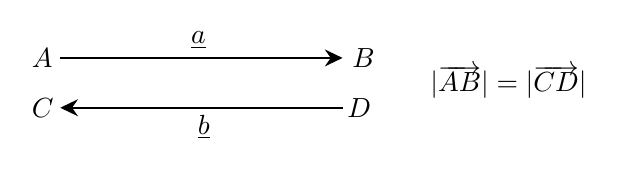
\begin{tikzpicture}[x=0.75pt,y=0.75pt,yscale=-0.8,xscale=0.8]
%uncomment if require: \path (0,179); %set diagram left start at 0, and has height of 179

%Straight Lines [id:da4122672604500781] 
\draw    (220,80) -- (387,80) ;
\draw [shift={(390,80)}, rotate = 180] [fill={rgb, 255:red, 0; green, 0; blue, 0 }  ][line width=0.08]  [draw opacity=0] (10.72,-5.15) -- (0,0) -- (10.72,5.15) -- (7.12,0) -- cycle    ;
%Straight Lines [id:da2306946235955416] 
\draw    (390,110) -- (223,110) ;
\draw [shift={(220,110)}, rotate = 360] [fill={rgb, 255:red, 0; green, 0; blue, 0 }  ][line width=0.08]  [draw opacity=0] (10.72,-5.15) -- (0,0) -- (10.72,5.15) -- (7.12,0) -- cycle    ;

% Text Node
\draw (201,72.4) node [anchor=north west][inner sep=0.75pt]    {$A$};
% Text Node
\draw (301,112.4) node [anchor=north west][inner sep=0.75pt]    {$\underline{b}$};
% Text Node
\draw (297,62.4) node [anchor=north west][inner sep=0.75pt]    {$\underline{a}$};
% Text Node
\draw (391,102.4) node [anchor=north west][inner sep=0.75pt]    {$D$};
% Text Node
\draw (201,102.4) node [anchor=north west][inner sep=0.75pt]    {$C$};
% Text Node
\draw (394,72.4) node [anchor=north west][inner sep=0.75pt]    {$B$};
% Text Node
\draw (441,82.4) node [anchor=north west][inner sep=0.75pt]    {$|\overrightarrow{AB}|=|\overrightarrow{CD}|$};


\end{tikzpicture}